\section{Design Reference}

\begin{figure}[!htbp]
	\centering
		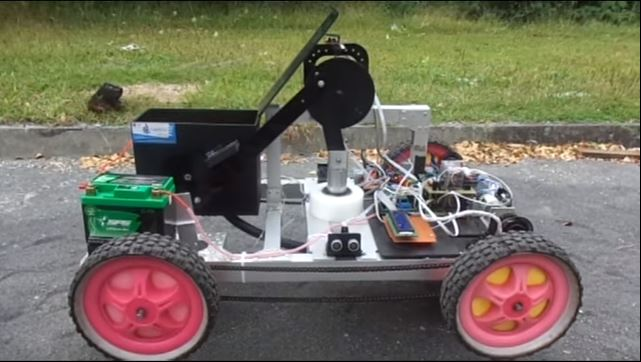
\includegraphics[width=0.5\textwidth]{Capture}
	\caption{Design Reference for The Corn Planting Robot}
	\label{fig:reference}
\end{figure}

Figure \ref{fig:reference} shows the researchers’ design reference for the corn planting robot. The design was found online (youtu.be/QooHpnYLj1w) which is uploaded by user named Luthfi Hasni. The design uses a PIC or a Programmable Integrated Circuit to control the robot. It uses several sensors as its navigation system. Besides from the 2 motors that controls the wheels of the robot, it has a third motor that controls the boring of the soil and the sowing of the cord seeds at the same time. 

\section{Design and Dimensions}

\begin{figure}[!htbp]
	\centering
		
\includegraphics[width=0.5\textwidth]{Design}
	\caption{System Design Diagram}
	\label{fig:Design}
\end{figure}

\begin{figure}[!htbp]
	\centering
		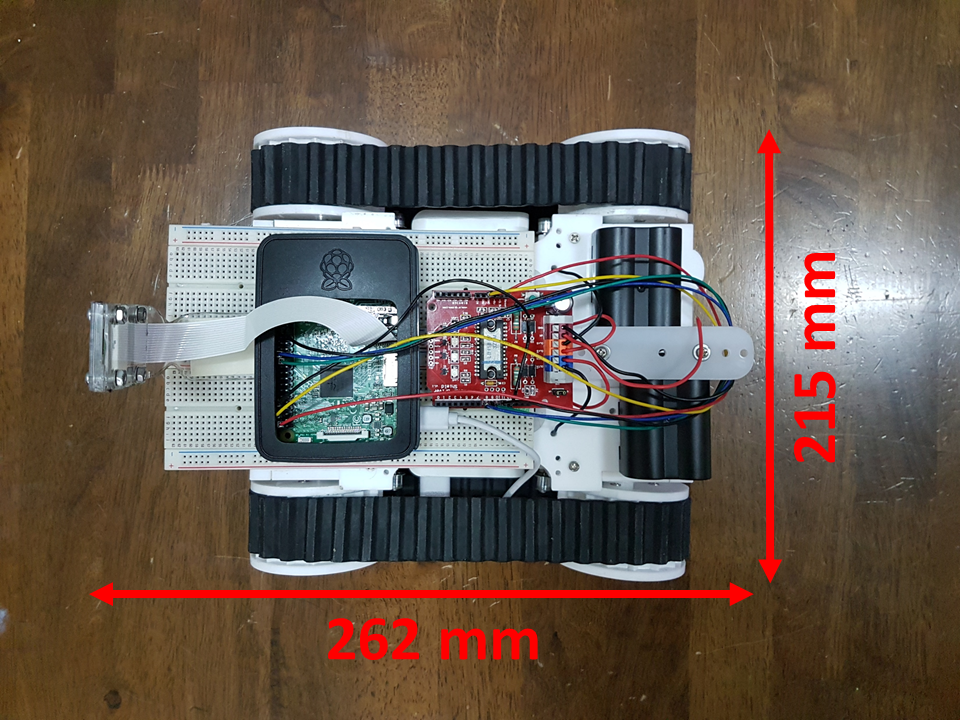
\includegraphics[width=0.5\textwidth]{2}
	\caption{Top View of the Corn Planting Robot and its Dimensions}
	\label{fig:1}
\end{figure}

\begin{figure}[!htbp]
	\centering
		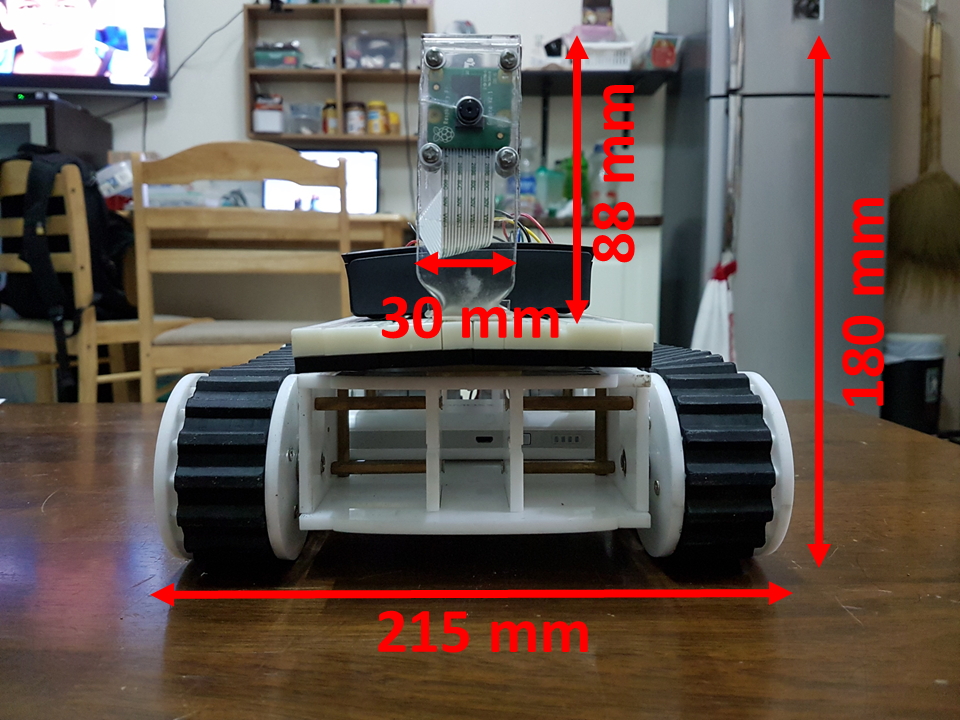
\includegraphics[width=0.5\textwidth]{3}
		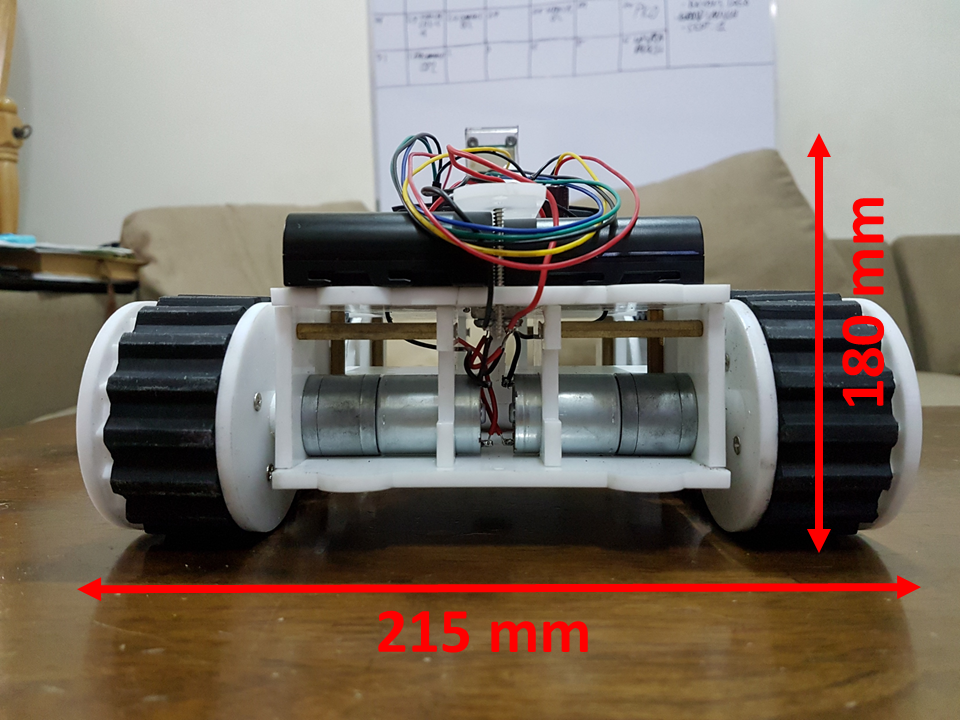
\includegraphics[width=0.5\textwidth]{4}
	\caption{Front and Back View of the Corn Planting Robot and its Dimensions}
	\label{fig:2}
\end{figure}

\begin{figure}[!htbp]
	\centering
		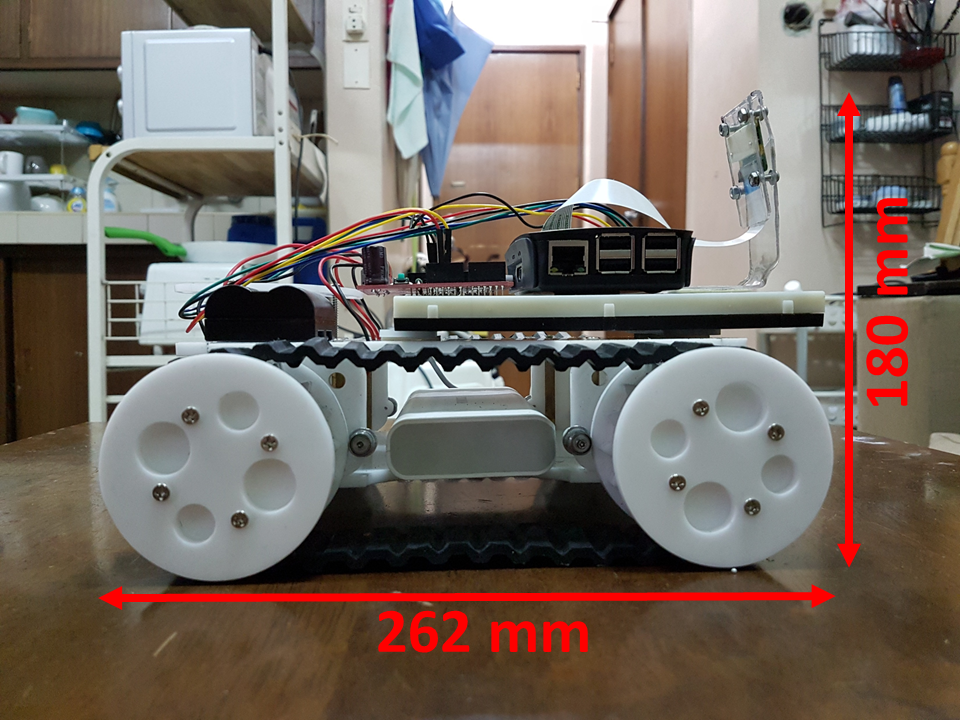
\includegraphics[width=0.5\textwidth]{5}
		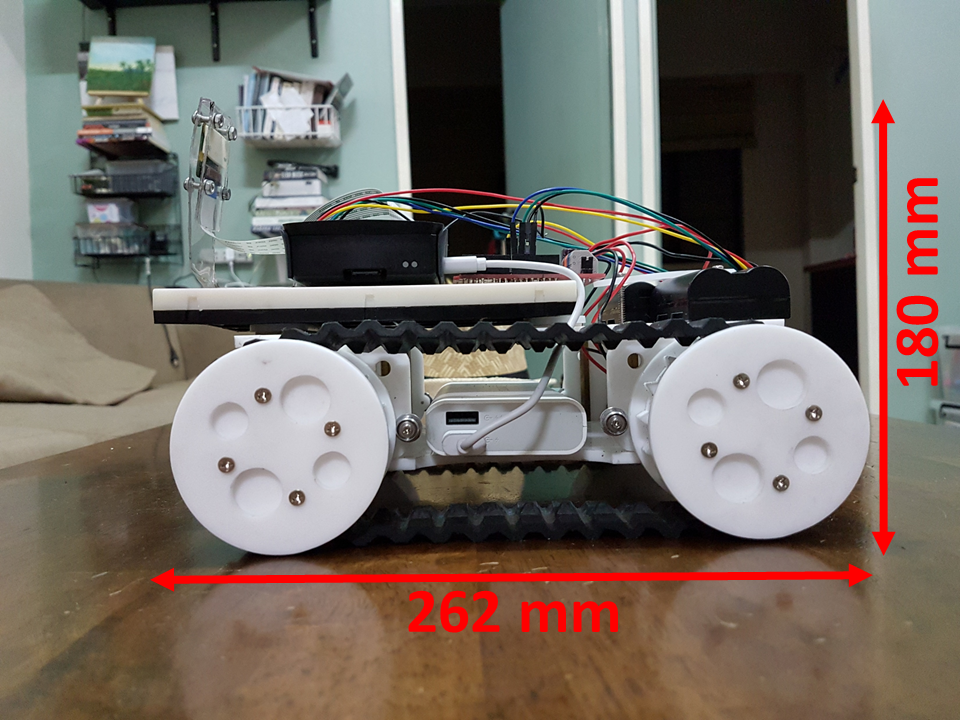
\includegraphics[width=0.5\textwidth]{6}
	\caption{Left and Right Side View of the Corn Planting Robot and its Dimensions}
	\label{fig:3}
\end{figure}

Portability is one of the main considerations of the robot’s design. Figures \ref{fig:1} - \ref{fig:3} shows the design and dimensions of the corn planting robot. The figures show that the researchers’ robot is much smaller compared to the design reference. The robot has a length of 262 mm, a width of 215 mm, and a height of 180 mm.

\section{Components}
\begin{figure}[!htbp]
	\centering
		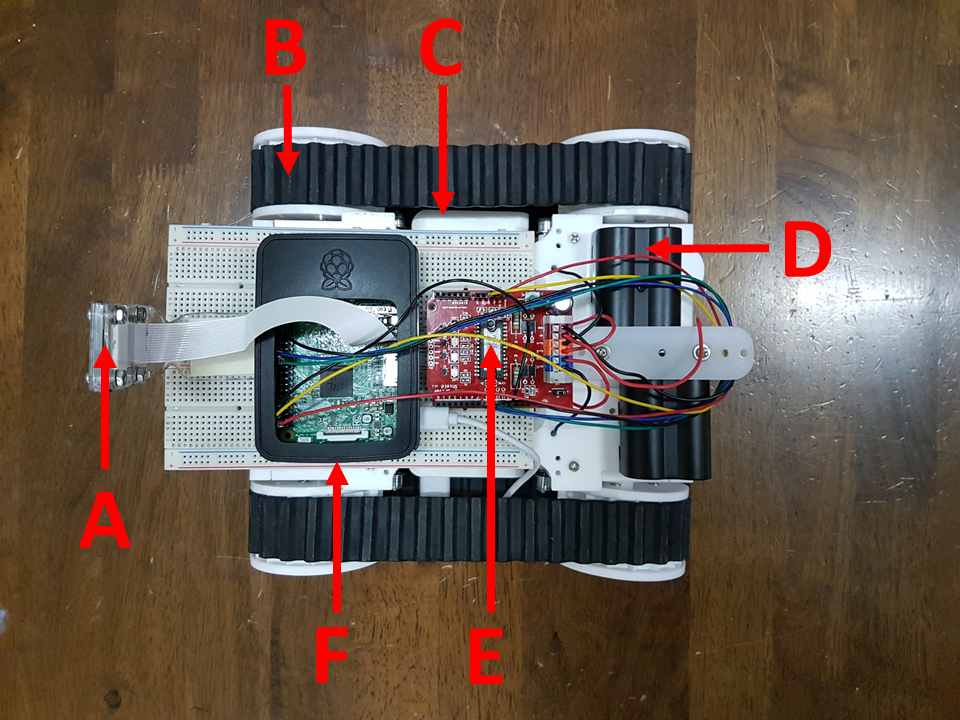
\includegraphics[width=0.5\textwidth]{1}
	\caption{Top View of the Corn Planting Robot with its Main Components Pointed Out}
	\label{fig:4}
\end{figure}

As seen on Figure \ref{fig:4}, part B is the continuous track of the robot. The researchers chose to use a continuous track for the robot since it is more suitable to be used on off-road environments on which corn in planted. The continuous track will help on the slip of the robot on the soil and help with the mobility of the robot.  The robot uses a 6V DC geared motor which controls the continuous track (B) which makes the robot move. Two 7.4 V battery packs (D) that is connected in parallel is used to supply voltage to the motors.  The motors and the battery packs (D) are then connected to the motor driver shield (E) which controls the direction of the motors individually thereby controls the movement of the whole robot. The motor driver shield is connected to the Raspberry Pi 3 Model B (F). The Raspberry Pi is the main processing unit of the robot. It is responsible for the image processing, remote connection, and the control of the motor driver shield (E). For the image processing, the researchers’ used the Raspberry Pi Camera v2.1 (A). We used the Raspberry Pi Camera for it allows the robot to utilize the GPU (Graphical Processing Unit) of the Raspberry Pi, which makes the image processing faster and decrease the processing load on the main processing unit. Lastly, the Raspberry Pi is then powered separately by a power bank.

	The researchers’ decided to use the Raspberry Pi instead of PIC or Arduino and other development boards due to its high processing ability, especially on image processing. PIC and Arduino are more suitable for applications that uses analog sensors or is more focused on hardware projects while the Raspberry Pi is more suitable for software processing. Since the corn planting robot would use computer vision to navigate across the corn field, the Raspberry Pi is more suitable for this kind of application. With a dedicated camera module that is directly compatible and can be easily set up, and a GPU or a Graphical Processing Unit, the Raspberry Pi can do image processing a lot faster which would allow the robot to do real time image processing and navigate across the field at the same time.
